% Results and discussion (R5: condensed from R1 by Vaishak and R2-R4 by Sanika).
% 5-seed numbers: scripts/aggregate_seeds.py + make_methods_tables.py (tab_grid,
% fig_corruption) and make_report_figures.py (fig_projection, fig_kpca left); seed-0 numbers:
% run_analysis.py, run_dtw.py, run_tuning.py.

\section{Results and Discussion}\label{sec:results}

\subsection{Leakage, model comparison and the projections}

\begin{table*}[t]
  \centering
  \caption{Grouped cross-validation: macro-F1 of every front-end and classifier (mean
  $\pm$ std over 5 seeds; chance 0.17). Bold: best.}
  \label{tab:grid}
  \begin{tabular}{lcccccc}
\toprule
Front-end & $k$-NN & $k$-NN (Mah.) & Lin.\ SVM & RBF SVM & RF & GNB \\
\midrule
Raw 126-D & 0.28 $\pm$ 0.03 & 0.25 $\pm$ 0.04 & \textbf{0.47 $\pm$ 0.03} & 0.35 $\pm$ 0.04 & 0.39 $\pm$ 0.05 & 0.27 $\pm$ 0.02 \\
PCA (95\% var.) & 0.29 $\pm$ 0.01 & 0.30 $\pm$ 0.03 & 0.41 $\pm$ 0.02 & 0.38 $\pm$ 0.03 & 0.40 $\pm$ 0.03 & 0.27 $\pm$ 0.06 \\
PCA-5 & 0.28 $\pm$ 0.03 & 0.23 $\pm$ 0.01 & 0.31 $\pm$ 0.04 & 0.36 $\pm$ 0.04 & 0.29 $\pm$ 0.04 & 0.24 $\pm$ 0.03 \\
LDA-5 & 0.45 $\pm$ 0.06 & 0.42 $\pm$ 0.06 & 0.44 $\pm$ 0.07 & 0.43 $\pm$ 0.05 & 0.42 $\pm$ 0.05 & 0.43 $\pm$ 0.06 \\
Kernel PCA-5 & 0.15 $\pm$ 0.01 & 0.16 $\pm$ 0.02 & 0.28 $\pm$ 0.05 & 0.20 $\pm$ 0.02 & 0.21 $\pm$ 0.06 & 0.21 $\pm$ 0.03 \\
\bottomrule
\end{tabular}

\end{table*}

\begin{figure*}[t]
  \centering
  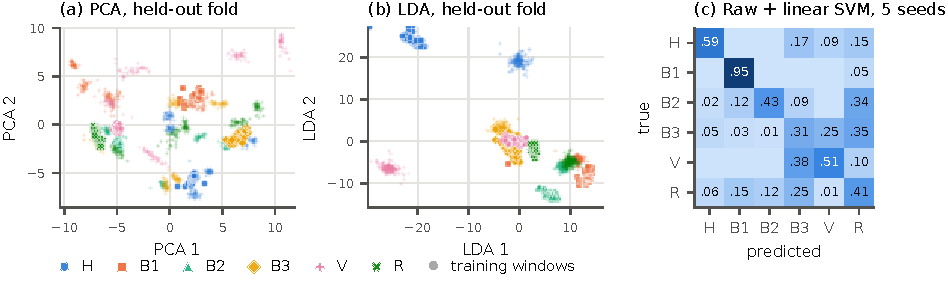
\includegraphics[width=\textwidth]{figures/fig_projection.pdf}
  \caption{(a, b) PCA and LDA fitted on one grouped fold's training recordings (small dots); large
  markers: the six held-out recordings, which land beside LDA's tight training clusters, not in
  them. (c) Row-normalised confusion matrix of the best model, pooled over 5 seeds.}
  \label{fig:projection}
\end{figure*}

\begin{figure*}[t]
  \centering
  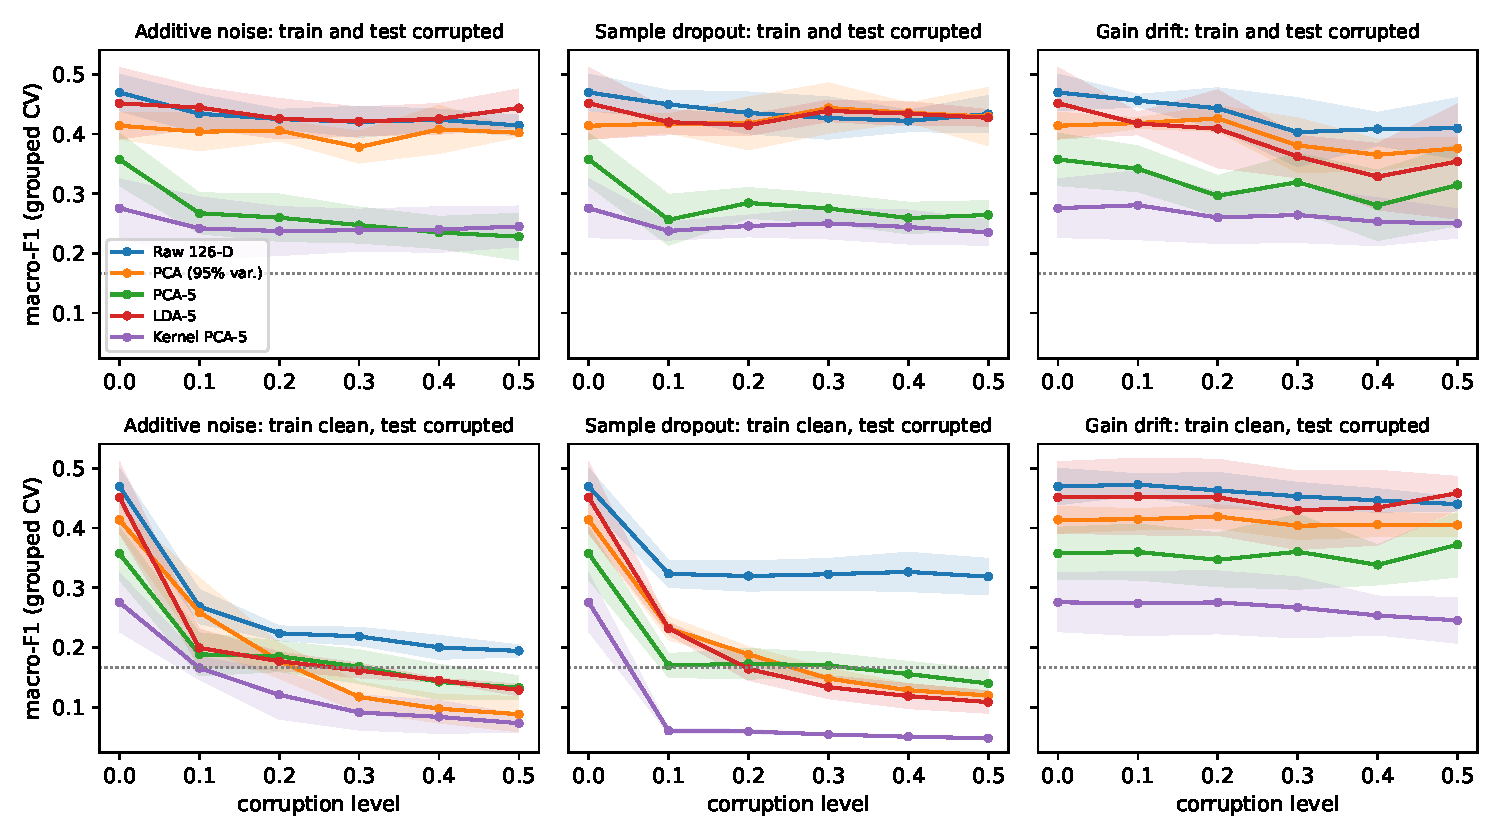
\includegraphics[width=0.6\textwidth]{figures/fig_corruption.pdf}
  \caption{Best macro-F1 per front-end against corruption level (grouped CV, 5 seeds, $\pm$1 std).
  Top: training and test corrupted alike; bottom: clean training, corrupted test; dotted: chance.}
  \label{fig:corruption}
\end{figure*}

Holding out whole recordings matters most: under the naive split 26 of the 30 models
score 0.99 or higher; with whole recordings held out none exceeds 0.47
(Table~\ref{tab:grid}), and leaving one condition out gives at most 0.56. The best model is the
linear SVM on the raw features ($0.47 \pm 0.03$). A max-margin linear boundary can combine many
weak cues across all 126 features, while the distance-based $k$-NN does poorly on the raw space
(0.25--0.28), where every feature counts equally, and well after LDA (0.42--0.45), which
reweights features by class separation. LDA-5 is decent with every classifier but not ahead over five
seeds (its seed-0 best, 0.49 with a random forest, does not hold). Separability on the training data misleads: LDA's Fisher $J$ at $k=5$ is about 490 in-sample but $15.1 \pm 4.7$ on held-out recordings, against $10.1 \pm 3.5$ for PCA. Most of what it
separates on its training fold is which recording a window came from (Fig.~\ref{fig:projection}b).
Per class (Fig.~\ref{fig:projection}c), B1 is recognised almost perfectly (recall 0.95), while H,
B3 and V blur together, and B2 is often taken for R (0.34).

\subsection{What survives a 100\,Hz sensor}\label{sec:separability}

Scored per class pair along the two-class LDA direction, the held-out $J$ is 0.4--7.4 against
600--1{,}600 in-sample. \textbf{B1 separates from every class} ($J$ 2.2--7.4), and against H
through impulsiveness: kurtosis ($J = 7.5$), peak-to-peak (4.7) and impulse factor (4.1). Poor
lubrication makes the vibration impulsive, and time-domain statistics capture that without any
defect frequency. No single feature separates any class from all five others (best weakest-pair $J$: 0.76).

\textbf{R is not separated by its rotor-bar sidebands,} the textbook broken-bar signature
\cite{nandi2005}. The sideband feature integrates
0.5--3\,Hz either side of $f_1$, but the measured pole-pass spacing is 3.5--10.1\,Hz under load
and below 0.5\,Hz unloaded, so it misses the real sidebands in all 36 recordings. Measured
directly, R's sidebands are never the strongest at their condition (rank 3, 6 and 4 of 6 under
load). At 50\,Hz supply they also coincide exactly with aliased shaft harmonics, for any slip:
for a four-pole motor $f_1 + f_p = 100 - 3f_1$, the alias of $3f_1$, and $f_1 - f_p$ is the alias
of $5f_1$. A 100\,Hz sensor cannot tell them apart. R's one consistent cue is slip under load
(median 0.056 against 0.043--0.047 for H and the bearing classes), hence the R$\leftrightarrow$B2
confusion.

\textbf{B3 and V} are defined by frequencies above Nyquist. Twice the line frequency folds to DC
at 50\,Hz supply and onto $f_1$ at 40\,Hz. H and V are best told apart by the energy at
\emph{aliased shaft-harmonic} positions ($J = 2.75$), mechanical harmonics folded down from above
50\,Hz, and V slips most under load (median 0.101). No spectral region separates B3 from H
($J \le 0.21$); its best single feature is skewness ($J = 1.11$), a waveform asymmetry rather
than a spectral line. These numbers are seed 0.

\subsection{Sensor corruption and unseen conditions}

The two deployments behave in opposite ways (Fig.~\ref{fig:corruption}). Corrupted alike,
noise and dropout barely matter even at 50\%. Gain drift hurts, and it hurts LDA most ($0.45 \to 0.35$ at level 0.5), because
the per-recording gain breaks the absolute amplitude cues LDA relies on. Trained clean, the
picture reverses: 10\% noise or dropout drops every projected front-end to 0.17--0.26 and Kernel
PCA to 0.06--0.17, while gain drift barely matters, since most features are scale-free ratios.
The raw features degrade least (0.32 at every dropout level). Corruption shifts the feature distribution (kurtosis, spectral kurtosis, entropy) rather than
erasing the classes, and projections fitted on clean data are the most
brittle to that shift, Kernel PCA most of all.

A new speed is easy: trained on 30 and 50\,Hz, the best model reaches $0.66 \pm 0.02$ at 40\,Hz.
A new load is the hard shift, because loading lowers the shaft speed and moves the whole harmonic
comb. Both PCA front-ends fall to 0.14--0.15 and Kernel PCA to 0.05; the raw features and LDA-5
keep about 0.40. B1 survives the load change (recall 0.92) while R falls to 0.16: its
load-dependent slip was never seen in training. Adaptation lifts the unseen load from 0.14--0.18
to 0.42--0.60, mostly through z-scoring each domain with its own statistics; Subspace Alignment
adds little and in either direction ($-0.07$ to $+0.09$ against z-scoring). The shift is mostly
a change of location and scale per feature.

\subsection{Kernel PCA, tuning and DTW}

\begin{figure}[t]
  \centering
  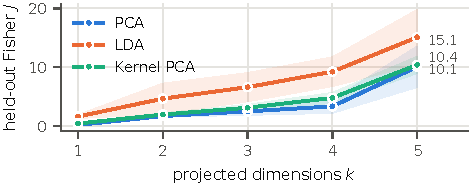
\includegraphics[width=\columnwidth]{figures/fig_fisher_k.pdf}
  \caption{Held-out Fisher $J$ against $k$ (5 seeds, mean $\pm$ std).}
  \label{fig:kpca}
\end{figure}

The non-linear projection does not help. Kernel PCA keeps as much held-out separability as PCA
at every $k$ ($10.4 \pm 1.5$ against $10.1 \pm 3.5$ at $k=5$; Fig.~\ref{fig:kpca}), yet its best
classifier reaches only $0.28 \pm 0.05$. With $\gamma = 1/126$, two standardised windows sit
about 16 apart, where the kernel is already down to 0.13, so the embedding emphasises local
neighbourhoods of the training recordings. Consistent with that, nested tuning most often picks
the wider $\gamma = 0.002$, which brings Kernel PCA closer to linear PCA. Tuning in general changes
little (seed 0, every second training window): on the raw and LDA-5 front-ends the gain over
the defaults lies between $-0.03$ and $+0.04$, inside the fold-to-fold spread of 0.10--0.17, and
for most models the selected setting changes from fold to fold. The largest gain, Kernel PCA-5
with an RBF SVM (0.22 to 0.35),
still leaves it below the linear front-ends. Elastic alignment brings nothing either: DTW on the
window envelopes scores $0.28 \pm 0.07$ against $0.26 \pm 0.09$ without warping and
$0.30 \pm 0.12$ for the features (seed 0): windows of a steady run start at arbitrary shaft
phases, so there is nothing to align. The envelope beats the features on R (recall 0.61 against 0.23)
but not on B1 (0.54 against 0.97).
